% Created 2025-05-14 Wed 11:48
% Intended LaTeX compiler: lualatex
\documentclass[11pt, letterpaper]{article}
\usepackage{amsmath}
\usepackage{fontspec}
\usepackage{graphicx}
\usepackage{longtable}
\usepackage{wrapfig}
\usepackage{rotating}
\usepackage[normalem]{ulem}
\usepackage{capt-of}
\usepackage{hyperref}
\usepackage{parskip}
\usepackage{amsmath}
\usepackage{amssymb}
\usepackage[all]{foreign}
\usepackage{hyperref}
\hypersetup{colorlinks=true, linkcolor=blue}
\usepackage{caption}
\usepackage{mismath}
\usepackage{bm}
\usepackage{amssymb}
\usepackage{tikz}
\usetikzlibrary{fit, positioning}
\usepackage{xcolor}
\usepackage{booktabs}
\author{Andrea Pierré \\
}
\date{\today}
\title{CMP\\\medskip
\large Composition of Movement Primitives}
\hypersetup{
 pdfauthor={Andrea Pierré \\
},
 pdftitle={CMP},
 pdfkeywords={},
 pdfsubject={},
 pdfcreator={Emacs 30.1 (Org mode 9.7.27)}, 
 pdflang={English}}
\begin{document}

\maketitle
\tableofcontents

\section{ProMPs}
\label{sec:org14f8ef7}
\subsection{Recap}
\label{sec:org9ff910b}
\begin{itemize}
\item \(q_t\): joint angle over time
\item \(\dot{q}_t\): joint velocity over time
\item \(\bm{\tau} = \{q_t\}_{t=0\dots T}\): trajectory
\item \(\bm{w}\): weight vector of a single trajectory
\item \(\phi_t\): basis function
\item \(\bm{\Phi}_t = [\phi_t, \dot{\phi_t}]\): \(n \times 2\) dimensional time-dependent basis matrix
\item \(z(t)\): monotonically increasing phase variable
\item \(\bm{\epsilon}_y \sim \mathcal{N}(\bm{0}, \bm{\Sigma}_y)\): zero-mean i.i.d. Gaussian noise
\end{itemize}

\begin{gather}
\bm{y}_t = \begin{bmatrix}
       q_t \\[0.3em]
       \dot{q}_t
     \end{bmatrix} = \bm{\Phi}^{\top}_{t}\bm{w} + \bm{\epsilon}_y\\
p(\bm{\tau}|\bm{w}) = \prod_t \mathcal{N}\Big(\bm{y}_t|\bm{\Phi}^{\top}_{t}\bm{w}, \bm{\Sigma}_y \Big)\\
p(\bm{\tau};\bm{\theta}) = \int p(\bm{\tau}|\bm{w}) \cdot p(\bm{w};\bm{\theta}) d\bm{w}\label{eq:HBM}
\end{gather}
Equation \ref{eq:HBM} is illustrated in Figure \ref{fig:HBM}.

\begin{figure}[htbp]
\centering
\begin{tikzpicture}
\tikzstyle{main}=[circle, minimum size = 10mm, thick, draw =black!80, node distance = 16mm]
\tikzstyle{connect}=[-latex, thick]
\tikzstyle{box}=[rectangle, draw=black!100]
  \node[circle, draw=black!100, fill = black!10] (theta) [label=above:$\bm{\theta}$] { };
  \node[main] (w) [right=of theta,label=above:$p(\bm{w};\bm{\theta})$] {$\bm{w}$};
  \node[main] (y) [right=of w,label=above:$p(\bm{y}_t|\bm{w})$] {$\bm{y}_t$};
  \path (theta) edge [connect] (w)
		(w) edge [connect] (y);
  \node[rectangle, inner sep=1.5mm, fit= (y),label=below:{$t=1 \dots T$}] (ghost) {};
  \node[rectangle, rounded corners=0.2cm, inner sep=4.4mm,draw=black!100, fit= (y) (ghost)] {};
\end{tikzpicture}
\caption{Hierarchical Bayesian model used in ProMPs.}
\label{fig:HBM}
\end{figure}
\subsection{Coupling between joints}
\label{sec:org677edc1}
\begin{equation}
p(\bm{y}_t|\bm{w}) = \mathcal{N}\Bigg(
        \begin{bmatrix}
                \bm{y}_{1,t} \\
                \vdots\\
                \bm{y}_{d,t} \\
        \end{bmatrix}
        \Bigg|
        \begin{bmatrix}
                \bm{\Phi}^{\top}_{t} & \cdots & \bm{0} \\
                \vdots &\ddots & \vdots\\
                \bm{0} & \cdots & \bm{\Phi}^{\top}_{t} \\
        \end{bmatrix}
        \bm{w}, \bm{\Sigma}_y
\Bigg) = \mathcal{N}\Big(\bm{y}_t|\bm{\Psi}_t\bm{w},\bm{\Sigma}_y \Big)
\end{equation}
with:
\begin{itemize}
\item \(\bm{w}=[\bm{w}^\top_1, \dots, \bm{w}^\top_n]^\top\): combined weight vector
\item \(\bm{\Phi}_t\): block-diagonal basis matrix containing the basis functions and their derivatives for each dimension
\item \(\bm{y}_{i,t} = [q_{i,t}, \dot{q}_{i,t}]^\top\): joint angle and velocity for the \(i^{\text{th}}\) joint
\end{itemize}

\begin{align}
p(\bm{y}_t; \bm{\theta}) &= \int \mathcal{N}\Big(\bm{y}_t|\bm{\Psi}^\top_t \bm{w}, \bm{\Sigma}_y \Big) \cdot p(\bm{w}; \bm{\theta})\\
&= \int \mathcal{N}\Big(\bm{y}_t|\bm{\Psi}^\top_t \bm{w}, \bm{\Sigma}_y \Big) \cdot \mathcal{N}\Big(\bm{w}|\bm{\mu_w}, \bm{\Sigma_w} \Big) d\bm{w}\\
& \textcolor{red}{\dots\text{ToDo expand}\dots}\\
&= \mathcal{N}\Big( \bm{y}_t | \bm{\Psi}^\top_t \bm{\mu_w}, \bm{\Psi}^\top_t \bm{\Sigma_w} \bm{\Psi}_t + \bm{\Sigma}_y \Big)
\end{align}
\subsection{Via-Points Modulation}
\label{sec:orgab307f1}
\begin{itemize}
\item \(\bm{x}_t^\star = [\bm{y}_t^\star, \bm{\Sigma}^\star_t]\): desired observation
\item \(\bm{y}^\star_t\): desired position and velocity vector at time \(t\)
\item \(\bm{\Sigma}^\star_t\): accuracy of the desired observation
\end{itemize}

\begin{equation}
p(\bm{w}|\bm{x}_t^\star) \propto \mathcal{N}\Big( \bm{y}_t^\star | \bm{\Psi}_t^\top\bm{w}, \bm{\Sigma}^\star_t \Big) \cdot p(\bm{w})\label{eq:prob-cond-new}
\end{equation}

\begin{align}
& \textcolor{red}{\dots\text{ToDo expand}\dots}\\
\bm{\mu_w}^{[new]} &= \bm{\mu_w} + \bm{\Sigma_w}\bm{\Psi}_t \Big(\bm{\Sigma}_y^\star \bm{\Psi}_t^\top \bm{\Sigma_w}\bm{\Psi}_t \Big)^{-1} (\bm{y}_t^\star - \bm{\Psi}_t^\top \bm{\mu_w})\label{eq:mu-cond-new}\\
\bm{\Sigma_w}^{[new]} &= \bm{\Sigma_w} - \bm{\Sigma_w}\bm{\Psi}_t \Big(\bm{\Sigma}_y^\star \bm{\Psi}_t^\top \bm{\Sigma_w}\bm{\Psi}_t \Big)^{-1} \bm{\Psi}_t^\top \bm{\Sigma_w}\label{eq:sigma-cond-new}
\end{align}
\section{Gaussian Mixture Models recap}
\label{sec:org0cc01ae}
\begin{equation}
p(\bm{x}|\bm{\theta}) = \sum_{k=1}^K \pi_k p_k(\bm{x})
\end{equation}
\begin{itemize}
\item \(p_k\): \(k\text{th}\) mixture component
\item \(\pi_k\): mixture weights with \(0 \leq \pi_k \leq 1\) and \(\sum_{k=1}^K \pi_k = 1\)
\end{itemize}

\begin{equation}
p(\bm{x}) = \sum_{k=1}^K \pi_k \mathcal{N}(\bm{x}|\bm{\mu}_k, \bm{\Sigma}_k)
\end{equation}
\section{Composition of MPs}
\label{sec:orgecf2f7f}

From Figure \ref{schema}, we can compose a set of MPs by ``stitching'' them using the following mechanisms:
\begin{enumerate}
\item choosing appropriate via-points between each MP. One strategy is to define the via-point as the average between the ending MP and the starting one.
\item generating the MP using Equations \((\ref{eq:prob-cond-new})\), \((\ref{eq:mu-cond-new})\) and \((\ref{eq:sigma-cond-new})\), from \(z(t_{ini}) = \frac{i}{k}\) to \(z(t_{end}) = \frac{i+1}{k}\).
\end{enumerate}

\begin{figure}[htbp]
\centering
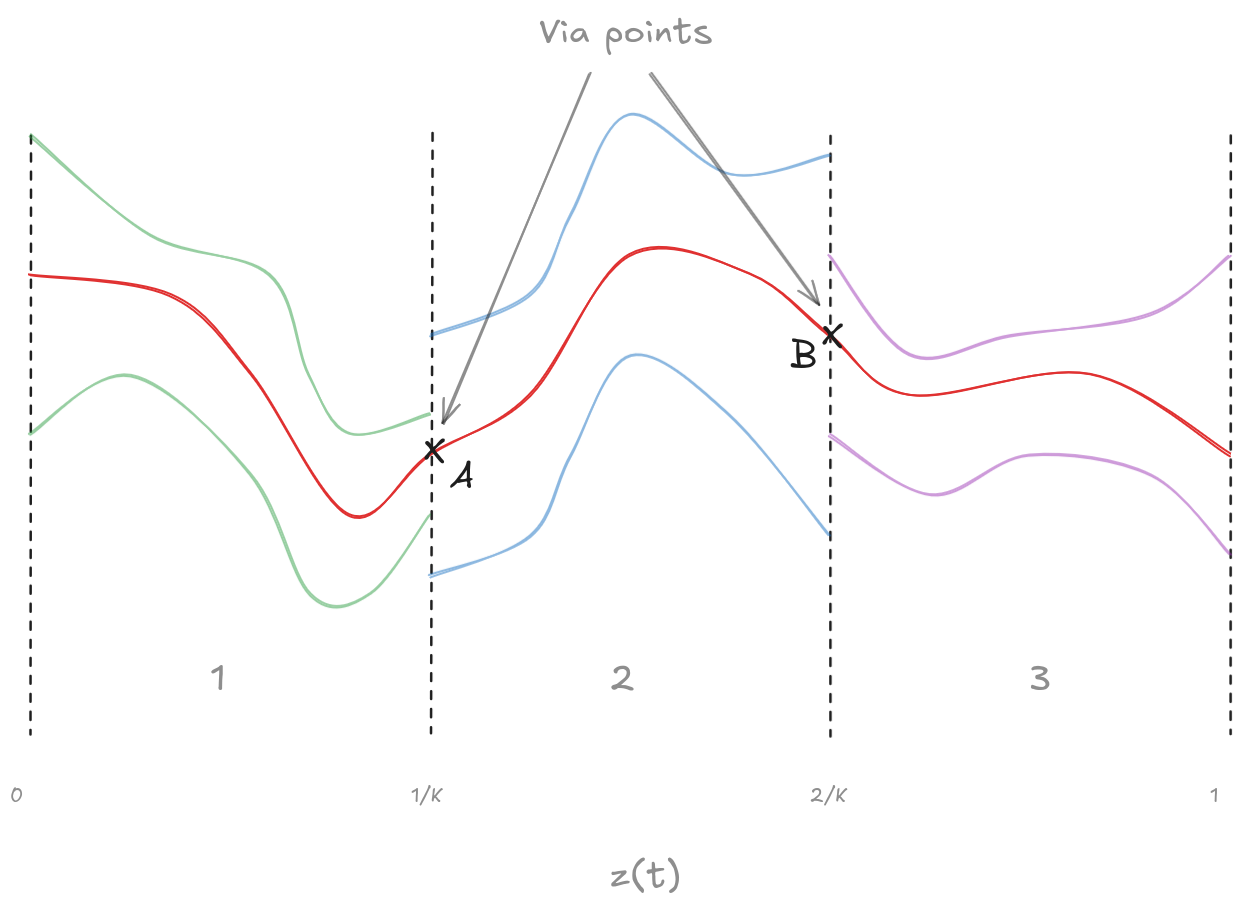
\includegraphics[width=0.9\textwidth]{fig/schema.png}
\caption{\label{schema}How to compose several ProMPs. Here \(K = 3\), and \(y_A = \frac{\mu_{1,t_A} + \mu_{2,t_A}}{2}; \quad y_B = \frac{\mu_{2,t_B} + \mu_{3,t_B}}{2}\).}
\end{figure}

Proposal on how to choose the via-points:
$$y_k = \frac{\mu_{k,t_{end}} + \mu_{k+1,t_{ini}}}{2}$$
$$\bm{y}_k = [\mu_{x_k}, \mu_{y_k}, \mu_{z_k},\dots]^\top$$
\[\bm{Y}_k =
 \begin{bmatrix}
       \mu_{x_1} & \mu_{y_1} & \mu_{z_1} & \cdots\\
       \vdots & \ddots &  & \vdots\\
       \mu_{x_k} & \mu_{y_k} & \mu_{z_k} & \cdots\\
     \end{bmatrix}
\]


A comparison of features available in MPs frameworks is available in Table \ref{feat-table}.
\begin{table}[htbp]
\begin{tabular}{lccccc}
\toprule
& DMP & ProMP & GMM & KMP & \textbf{CMP}\\
\midrule
Probabilistic & - & \checkmark & \checkmark & \checkmark & \checkmark\\
Via-point & - & \checkmark & - & \checkmark & \checkmark\\
End-point & \checkmark & \checkmark & - & \checkmark & \checkmark\\
Extrapolation & \checkmark & - & - & \checkmark & \textcolor{red}{Check KMP}\\
High-dimensional inputs & - & - & \checkmark & \checkmark & \textcolor{red}{Check KMP}\\
Composition & - & - & - & - & \checkmark\\
\bottomrule
\end{tabular}
\caption{Comparison of features available for each Movements Primitives frameworks.}
\label{feat-table}
\end{table}
\end{document}
